\documentclass[12pt,a4paper]{article}

\usepackage[utf8]{inputenc}
\usepackage[T1]{fontenc}
\usepackage{polski}

\usepackage{amsthm}
\usepackage{amsmath}
\usepackage{amsfonts}
\usepackage{amssymb}
\usepackage{pgfplots}
\usepackage{tikz}
\usepackage{lmodern}	%fancy font
\usepackage{textcomp}

\usepackage{graphicx}
\usepackage{caption}
\usepackage{subcaption}
\usepackage{here}


\setlength{\textheight}{24cm}
\setlength{\textwidth}{15.92cm}
\setlength{\footskip}{10mm}
\setlength{\oddsidemargin}{0mm}
\setlength{\evensidemargin}{0mm}
\setlength{\topmargin}{0mm}
\setlength{\headsep}{5mm}
\usepackage{tikz}
\usepackage{lmodern}	%fancy font
\usepackage{textcomp}

\usepackage{indentfirst}
\usepackage{graphicx}
\usepackage{caption}
\usepackage{subcaption}
%\usepackage{siunitx}
\usepackage{here}
\usepackage[margin=1in]{geometry}% Just for this example
\setlength{\textheight}{24cm}
\setlength{\textwidth}{15.92cm}
\setlength{\footskip}{10mm}
\setlength{\oddsidemargin}{0mm}
\setlength{\evensidemargin}{0mm}
\setlength{\topmargin}{0mm}


\begin{document}

\begin{table}[]
\label{my-label}
\begin{tabular}{|p{7.5cm}|p{7.5cm}|}
\hline
									           					&                           \\

\includegraphics[height=3cm]{logo}             					& \textbf{Technika cyfrowa} \\ \hline
\multicolumn{1}{|l|}{\textbf{Temat ćwiczenia}} 					& \textbf{Numer ćwiczenia}  \\
\multicolumn{1}{|l|}{Liczniki}	& 4                         \\ \hline
\multicolumn{1}{|l|}{\textbf{Wykonawca}}       & \textbf{Ocena}            \\
\multicolumn{1}{|l|}{Łukasz Nawojowski}          &                           \\ \hline
\end{tabular}
\end{table}

\section{Cel ćwiczenia}
Zaznajomienie się ze sposobami konstrukcji liczników przy użyciu przerzutników i bramek logicznych.

\section{Dwójka licząca}
Sporządzono tablice Karnaugh dla obu wersji licznika.
\begin{figure}[H]
\centering
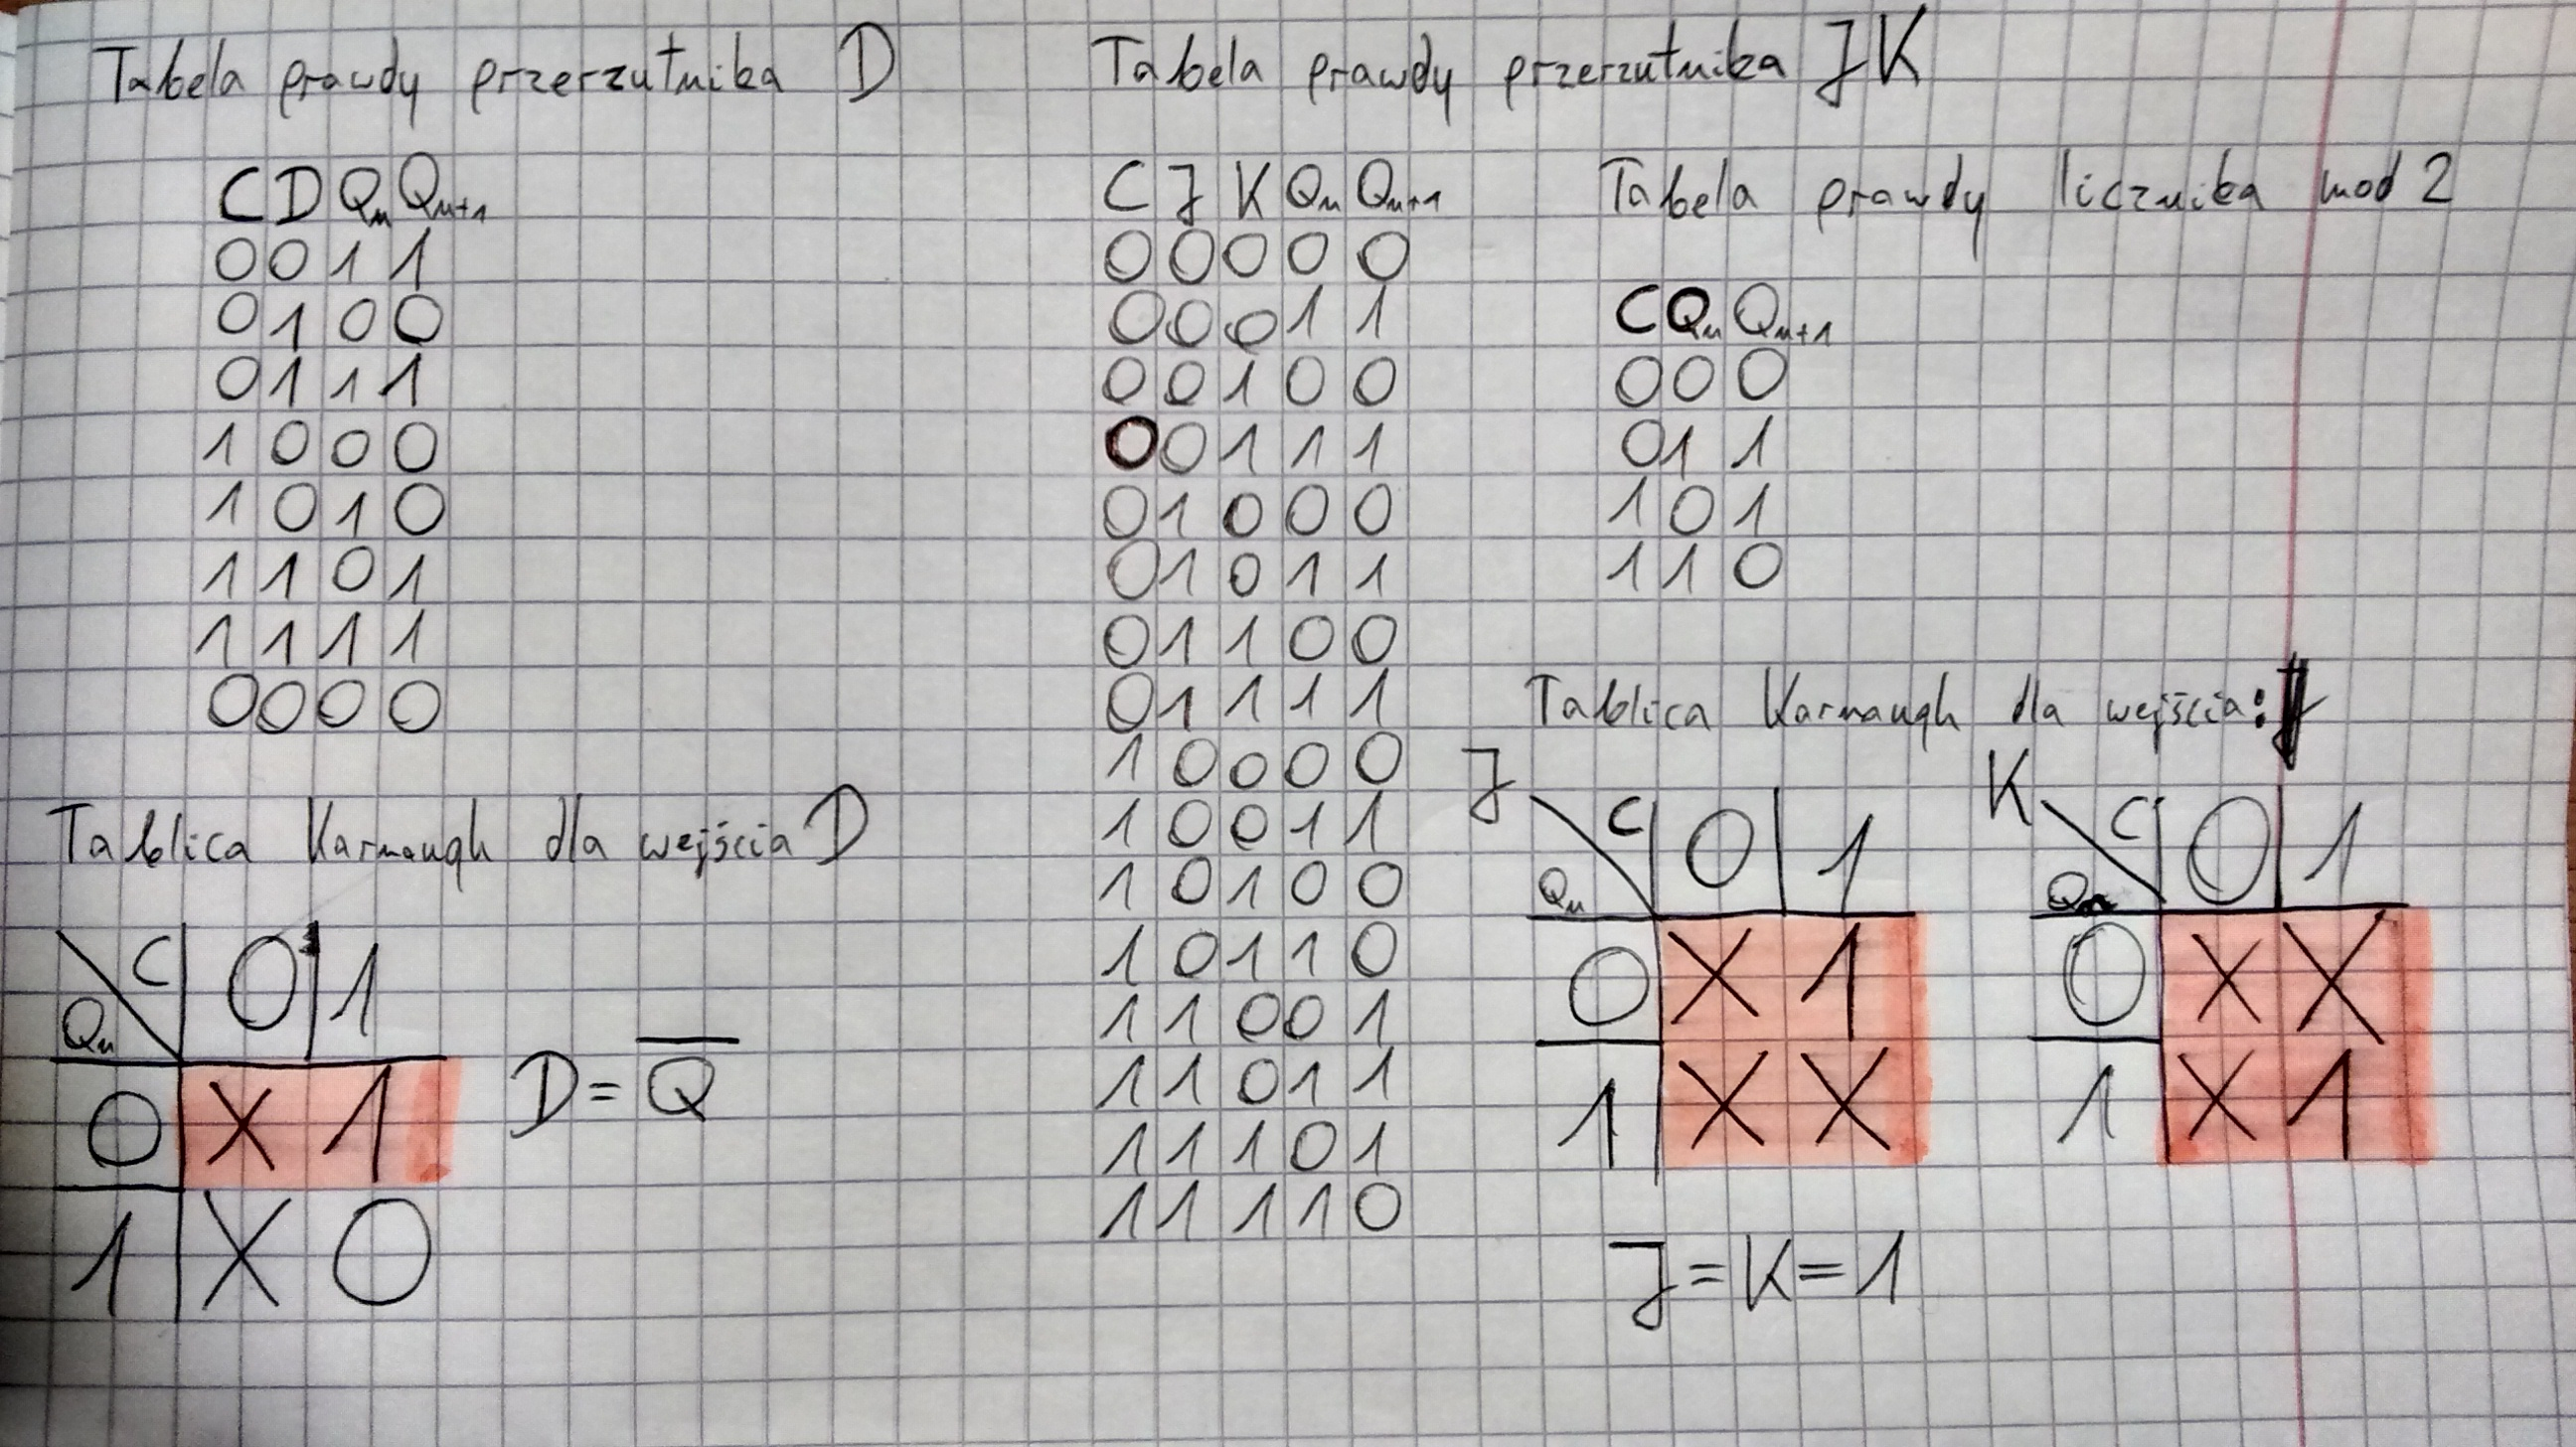
\includegraphics[width=\textwidth]{img/4a_tables}
\end{figure}

\newpage
Zbudowano odpowiadające im układy w Multisimie.
\begin{figure}[H]
\centering
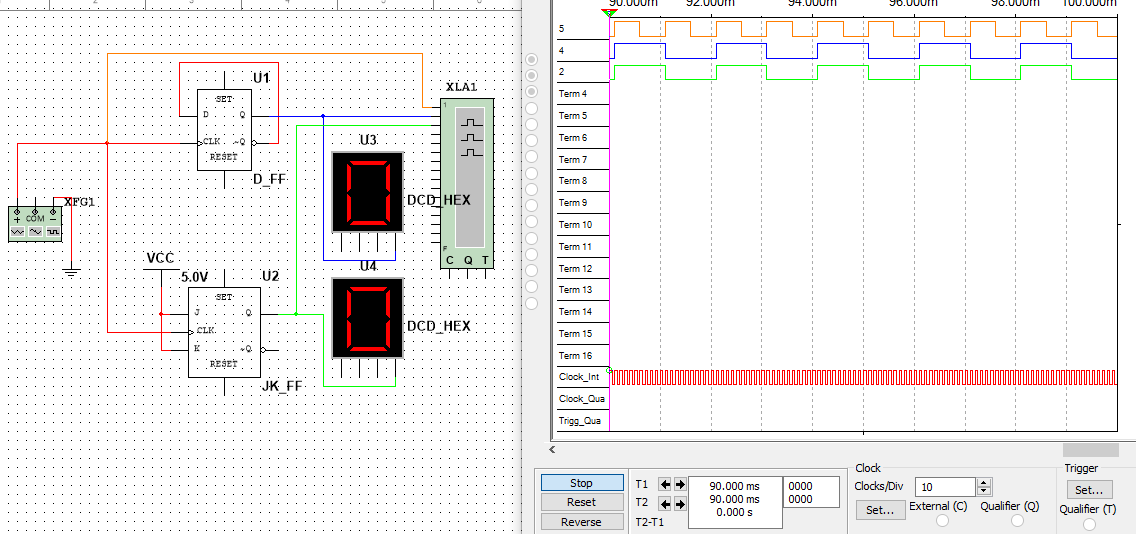
\includegraphics[width=\textwidth]{img/4a_circuit}
\end{figure}

Zaobserwowano prawidłowe działanie układów. Widzimy, że wyjście dwójki liczącej też jest zegarem, tyle że z okresem dwa razy dłuższym niż wejściowy, z czego skorzystamy przy budowie licznika asynchronicznego.


\section{Czterobitowy licznik asynchroniczny}
Przy budowie licznika czterobitowego skorzystałem z przerzutników T, których poznana wcześniej zasada działania wydała mi się optymalna do tego celu. Jeden przerzutnik odpowiada jednemu bitowi wyjścia. Korzystając z zaobserwowanego wcześniej faktu, że dwójka licząca daje sygnał zegarowy o okresie 2 razy dłuższym niż wejściowy, a każdy kolejny bit powinien przeskakiwać z 2 razy mniejszą częstotliwością niż poprzedni, aby uzyskać ten efekt, wystarczy połączyć wyjście każdego kolejnego przerzutnika z wejściem zegarowym kolejnego.

Na tej podstawie zbudowano układ w Multisimie.
\begin{figure}[H]
\centering
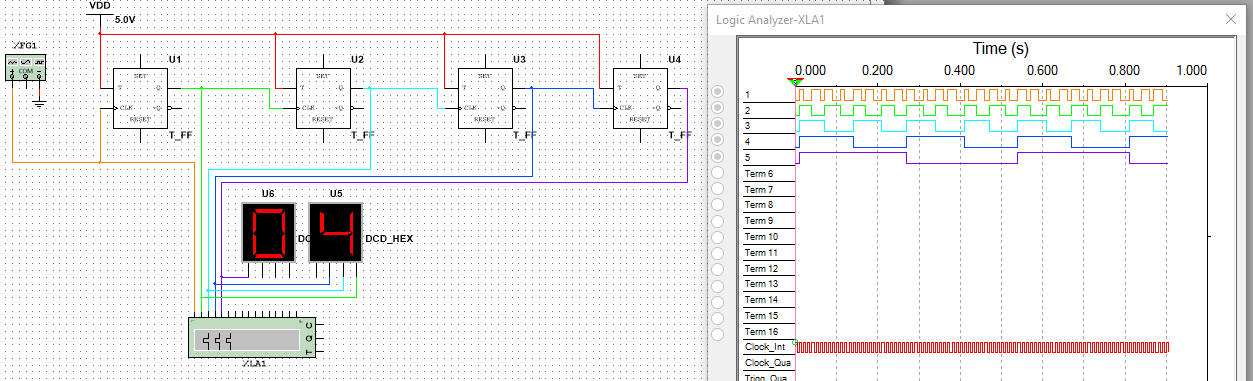
\includegraphics[width=\textwidth]{img/4b_circuit}
\end{figure}

Widzimy, że kolejne bity zmieniają się z 2 razy mniejszą częstością, a na ekranach pojawiają się kolejne cyfry (całkowite wskazanie licznika to suma liczb na obu ekranach), jednak licznik odlicza w dół. Aby to zmienić, wystarczy zanegować wejścia zegarowe każdego przerzutnika. O ile w przypadku najmłodszego bitu spowoduje to jedynie przesunięcie sygnału wyjściowego o połowę okresu, to w przypadku bitów starszych zmiana ma trochę inny charakter.

Po pierwsze, przerzutniki były wszystkie w tej samej pozycji początkowej 0. Początkowa zmiana najmłodszego bitu z 0 na 1 powodowała kaskadowe ustawienie wszystkich pozostałych bitów na 1. Po zanegowaniu sygnału zegarowego na każdym przerzutniku na samym początku zmienia się tylko bit najmłodszy, reszta pozostaje w pozycji 0, bo starsze bity reagują teraz na opadanie sygnału.

Po drugie, rozważmy 2 bity, starszy i młodszy, ustawione na 1. Jeśli starszy bit reaguje na zmianę młodszego bitu z 0 na 1 i opada wtedy na 0, to sumaryczne wskazanie licznika maleje, ponieważ opadający starszy bit ma 2 razy większą wartość niż wznoszący się bit młodszy. Odpowiada to licznikowi bez zanegowanych wejść zegarowych. Jeśli z kolei weźmiemy te bity oba ustawione na 0 i starszy bit reaguje na opadanie młodszego bitu z 1 na 0, to przy zmianie sumaryczne wskazanie licznika rośnie, bo wznoszący się starszy bit ma 2 razy większą wartość niż opadający bit młodszy, co odpowiada licznikowi z zanegowanymi wejściami zegarowymi. Przetestowano również tę drugą wersję licznika, która rzeczywiście liczy rosnąco.

\begin{figure}[H]
\centering
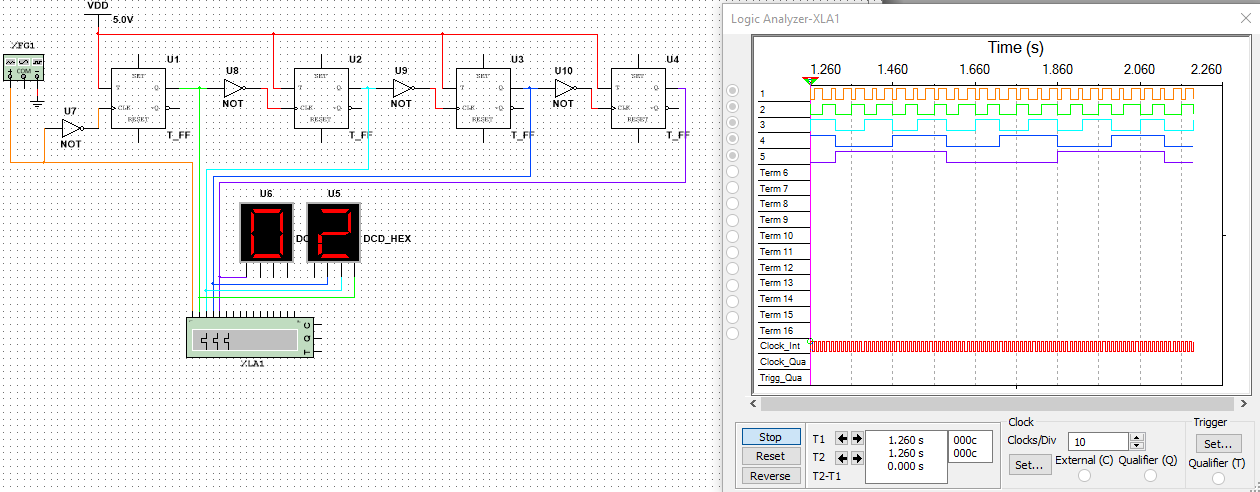
\includegraphics[width=\textwidth]{img/4b_circuit2}
\end{figure}

Podczas niektórych zmian cyfry na wyświetlaczu mrugały, co może mieć związek z tym, że sygnał propaguje się ze skończoną szybkością od najmłodszego do najstarszego bitu, co może generować pewne chwile, w których licznik jako całość przechodzi z jednego stanu w drugi.


\newpage
\section{Synchroniczny licznik mod 8}
$8 = 2^3$, zatem licznik będzie miał 3 wyjścia. Zauważmy, że wartości kolejnych starszych bitów zależą jedynie od swojej poprzedniej wartości oraz wartości bitów młodszych. Wyjście nie zależy również od sygnału zegarowego, który pełni jedynie rolę synchronizatora, co można już było zaobserwować przy budowie licznika mod 2. Na tej podstawie sporządzono tabele Karnaugh dla poszczególnych bitów, przy czym bit najmłodszy, to po prostu zwykły licznik mod 2.

\begin{figure}[H]
\centering
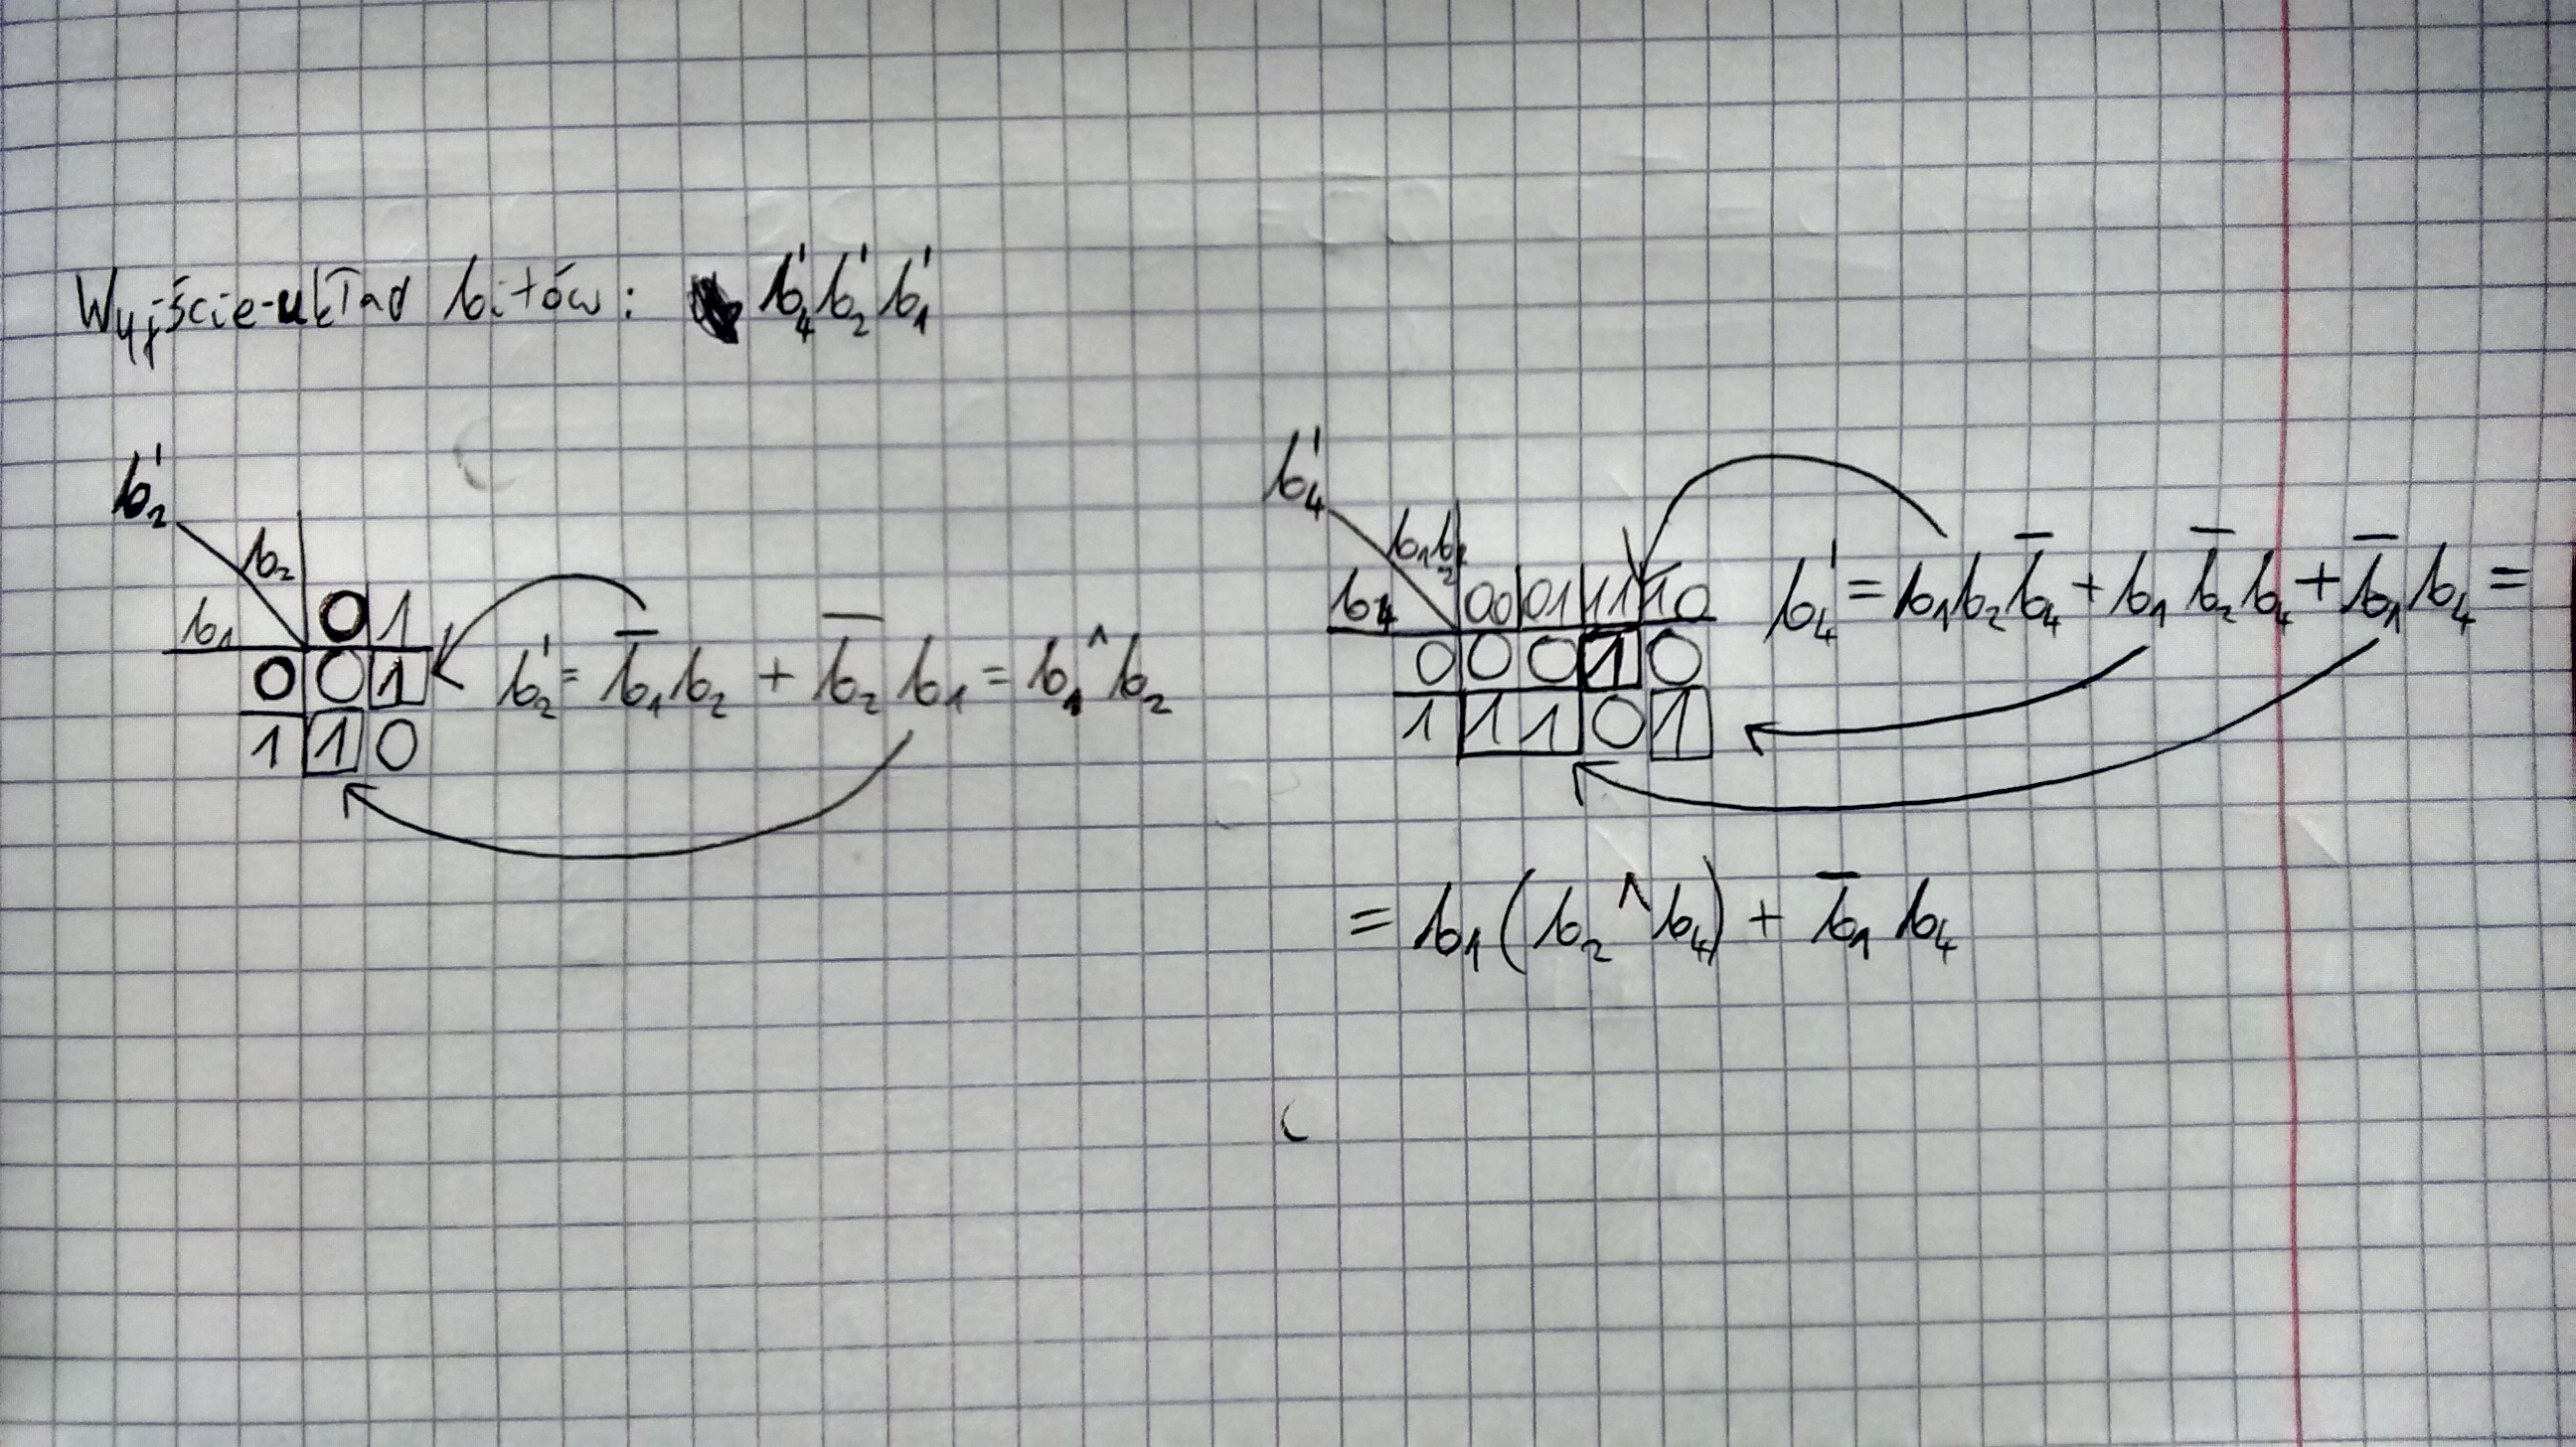
\includegraphics[width=\textwidth]{img/4c_tables}
\end{figure}

Na tej podstawie zbudowano układ w Multisimie.
\begin{figure}[H]
\centering
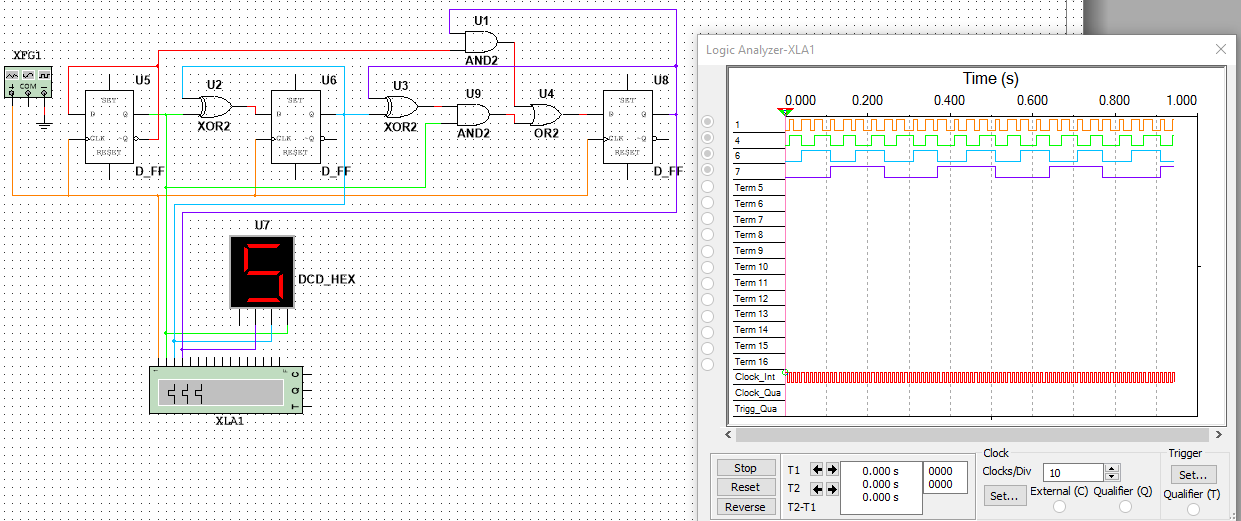
\includegraphics[width=\textwidth]{img/4c_circuit}
\end{figure}

I znów widzimy znajomy już układ sygnałów, co jest niechybną oznaką, że układ działa zgodnie z oczekiwaniami. Ten licznik jest synchroniczny, co pozwala na ustabilizowanie działania, jednak odbywa się to kosztem skomplikowania układu wewnętrznego licznika.


\section{Licznik mod 6}
Licznik mod 6 działa w zasadzie tak samo jak licznik czterobitowy mod 16, tyle że po osiągnięciu 6 wszystkie przerzutniki muszą być zresetowane. Możemy to osiągnąć łącząc koniunkcję bitów o wartości 2 i 4 z wejściami reset wszystkich przerzutników. Skorzystamy z asynchronicznego licznika zbudowanego wcześniej.

\begin{figure}[H]
\centering
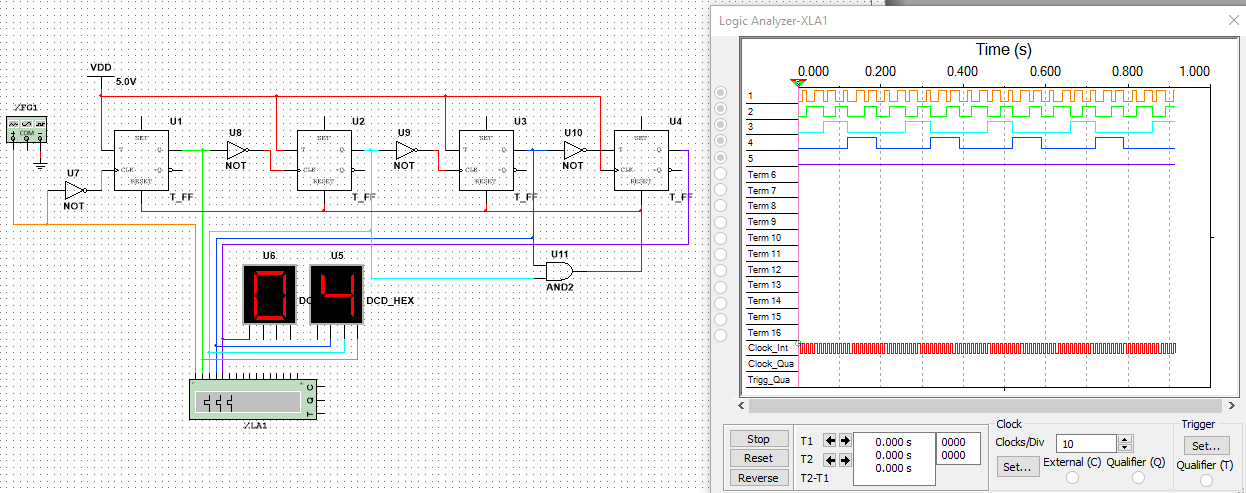
\includegraphics[width=\textwidth]{img/4d_circuit}
\end{figure}

Układ działa zgodnie z oczekiwaniami.

\end{document}
